%% template.tex
%% from
%% bare_conf.tex
%% V1.4b
%% 2015/08/26
%% by Michael Shell
%% See:
%% http://www.michaelshell.org/
%% for current contact information.
%%
%% This is a skeleton file demonstrating the use of IEEEtran.cls
%% (requires IEEEtran.cls version 1.8b or later) with an IEEE
%% conference paper.
%%
%% Support sites:
%% http://www.michaelshell.org/tex/ieeetran/
%% http://www.ctan.org/pkg/ieeetran
%% and
%% http://www.ieee.org/

%%*************************************************************************
%% Legal Notice:
%% This code is offered as-is without any warranty either expressed or
%% implied; without even the implied warranty of MERCHANTABILITY or
%% FITNESS FOR A PARTICULAR PURPOSE!
%% User assumes all risk.
%% In no event shall the IEEE or any contributor to this code be liable for
%% any damages or losses, including, but not limited to, incidental,
%% consequential, or any other damages, resulting from the use or misuse
%% of any information contained here.
%%
%% All comments are the opinions of their respective authors and are not
%% necessarily endorsed by the IEEE.
%%
%% This work is distributed under the LaTeX Project Public License (LPPL)
%% ( http://www.latex-project.org/ ) version 1.3, and may be freely used,
%% distributed and modified. A copy of the LPPL, version 1.3, is included
%% in the base LaTeX documentation of all distributions of LaTeX released
%% 2003/12/01 or later.
%% Retain all contribution notices and credits.
%% ** Modified files should be clearly indicated as such, including  **
%% ** renaming them and changing author support contact information. **
%%*************************************************************************


% *** Authors should verify (and, if needed, correct) their LaTeX system  ***
% *** with the testflow diagnostic prior to trusting their LaTeX platform ***
% *** with production work. The IEEE's font choices and paper sizes can   ***
% *** trigger bugs that do not appear when using other class files.       ***                          ***
% The testflow support page is at:
% http://www.michaelshell.org/tex/testflow/

\documentclass[conference,final,]{IEEEtran}
% Some Computer Society conferences also require the compsoc mode option,
% but others use the standard conference format.
%
% If IEEEtran.cls has not been installed into the LaTeX system files,
% manually specify the path to it like:
% \documentclass[conference]{../sty/IEEEtran}





% Some very useful LaTeX packages include:
% (uncomment the ones you want to load)


% *** MISC UTILITY PACKAGES ***
%
%\usepackage{ifpdf}
% Heiko Oberdiek's ifpdf.sty is very useful if you need conditional
% compilation based on whether the output is pdf or dvi.
% usage:
% \ifpdf
%   % pdf code
% \else
%   % dvi code
% \fi
% The latest version of ifpdf.sty can be obtained from:
% http://www.ctan.org/pkg/ifpdf
% Also, note that IEEEtran.cls V1.7 and later provides a builtin
% \ifCLASSINFOpdf conditional that works the same way.
% When switching from latex to pdflatex and vice-versa, the compiler may
% have to be run twice to clear warning/error messages.






% *** CITATION PACKAGES ***
%
%\usepackage{cite}
% cite.sty was written by Donald Arseneau
% V1.6 and later of IEEEtran pre-defines the format of the cite.sty package
% \cite{} output to follow that of the IEEE. Loading the cite package will
% result in citation numbers being automatically sorted and properly
% "compressed/ranged". e.g., [1], [9], [2], [7], [5], [6] without using
% cite.sty will become [1], [2], [5]--[7], [9] using cite.sty. cite.sty's
% \cite will automatically add leading space, if needed. Use cite.sty's
% noadjust option (cite.sty V3.8 and later) if you want to turn this off
% such as if a citation ever needs to be enclosed in parenthesis.
% cite.sty is already installed on most LaTeX systems. Be sure and use
% version 5.0 (2009-03-20) and later if using hyperref.sty.
% The latest version can be obtained at:
% http://www.ctan.org/pkg/cite
% The documentation is contained in the cite.sty file itself.






% *** GRAPHICS RELATED PACKAGES ***
%
\ifCLASSINFOpdf
  % \usepackage[pdftex]{graphicx}
  % declare the path(s) where your graphic files are
  % \graphicspath{{../pdf/}{../jpeg/}}
  % and their extensions so you won't have to specify these with
  % every instance of \includegraphics
  % \DeclareGraphicsExtensions{.pdf,.jpeg,.png}
\else
  % or other class option (dvipsone, dvipdf, if not using dvips). graphicx
  % will default to the driver specified in the system graphics.cfg if no
  % driver is specified.
  % \usepackage[dvips]{graphicx}
  % declare the path(s) where your graphic files are
  % \graphicspath{{../eps/}}
  % and their extensions so you won't have to specify these with
  % every instance of \includegraphics
  % \DeclareGraphicsExtensions{.eps}
\fi
% graphicx was written by David Carlisle and Sebastian Rahtz. It is
% required if you want graphics, photos, etc. graphicx.sty is already
% installed on most LaTeX systems. The latest version and documentation
% can be obtained at:
% http://www.ctan.org/pkg/graphicx
% Another good source of documentation is "Using Imported Graphics in
% LaTeX2e" by Keith Reckdahl which can be found at:
% http://www.ctan.org/pkg/epslatex
%
% latex, and pdflatex in dvi mode, support graphics in encapsulated
% postscript (.eps) format. pdflatex in pdf mode supports graphics
% in .pdf, .jpeg, .png and .mps (metapost) formats. Users should ensure
% that all non-photo figures use a vector format (.eps, .pdf, .mps) and
% not a bitmapped formats (.jpeg, .png). The IEEE frowns on bitmapped formats
% which can result in "jaggedy"/blurry rendering of lines and letters as
% well as large increases in file sizes.
%
% You can find documentation about the pdfTeX application at:
% http://www.tug.org/applications/pdftex

\usepackage{graphicx}

% *** MATH PACKAGES ***
%
%\usepackage{amsmath}
% A popular package from the American Mathematical Society that provides
% many useful and powerful commands for dealing with mathematics.
%
% Note that the amsmath package sets \interdisplaylinepenalty to 10000
% thus preventing page breaks from occurring within multiline equations. Use:
%\interdisplaylinepenalty=2500
% after loading amsmath to restore such page breaks as IEEEtran.cls normally
% does. amsmath.sty is already installed on most LaTeX systems. The latest
% version and documentation can be obtained at:
% http://www.ctan.org/pkg/amsmath





% *** SPECIALIZED LIST PACKAGES ***
%
%\usepackage{algorithmic}
% algorithmic.sty was written by Peter Williams and Rogerio Brito.
% This package provides an algorithmic environment fo describing algorithms.
% You can use the algorithmic environment in-text or within a figure
% environment to provide for a floating algorithm. Do NOT use the algorithm
% floating environment provided by algorithm.sty (by the same authors) or
% algorithm2e.sty (by Christophe Fiorio) as the IEEE does not use dedicated
% algorithm float types and packages that provide these will not provide
% correct IEEE style captions. The latest version and documentation of
% algorithmic.sty can be obtained at:
% http://www.ctan.org/pkg/algorithms
% Also of interest may be the (relatively newer and more customizable)
% algorithmicx.sty package by Szasz Janos:
% http://www.ctan.org/pkg/algorithmicx




% *** ALIGNMENT PACKAGES ***
%
%\usepackage{array}
% Frank Mittelbach's and David Carlisle's array.sty patches and improves
% the standard LaTeX2e array and tabular environments to provide better
% appearance and additional user controls. As the default LaTeX2e table
% generation code is lacking to the point of almost being broken with
% respect to the quality of the end results, all users are strongly
% advised to use an enhanced (at the very least that provided by array.sty)
% set of table tools. array.sty is already installed on most systems. The
% latest version and documentation can be obtained at:
% http://www.ctan.org/pkg/array


% IEEEtran contains the IEEEeqnarray family of commands that can be used to
% generate multiline equations as well as matrices, tables, etc., of high
% quality.




% *** SUBFIGURE PACKAGES ***
%\ifCLASSOPTIONcompsoc
%  \usepackage[caption=false,font=normalsize,labelfont=sf,textfont=sf]{subfig}
%\else
%  \usepackage[caption=false,font=footnotesize]{subfig}
%\fi
% subfig.sty, written by Steven Douglas Cochran, is the modern replacement
% for subfigure.sty, the latter of which is no longer maintained and is
% incompatible with some LaTeX packages including fixltx2e. However,
% subfig.sty requires and automatically loads Axel Sommerfeldt's caption.sty
% which will override IEEEtran.cls' handling of captions and this will result
% in non-IEEE style figure/table captions. To prevent this problem, be sure
% and invoke subfig.sty's "caption=false" package option (available since
% subfig.sty version 1.3, 2005/06/28) as this is will preserve IEEEtran.cls
% handling of captions.
% Note that the Computer Society format requires a larger sans serif font
% than the serif footnote size font used in traditional IEEE formatting
% and thus the need to invoke different subfig.sty package options depending
% on whether compsoc mode has been enabled.
%
% The latest version and documentation of subfig.sty can be obtained at:
% http://www.ctan.org/pkg/subfig




% *** FLOAT PACKAGES ***
%

%\usepackage{fixltx2e}
% fixltx2e, the successor to the earlier fix2col.sty, was written by
% Frank Mittelbach and David Carlisle. This package corrects a few problems
% in the LaTeX2e kernel, the most notable of which is that in current
% LaTeX2e releases, the ordering of single and double column floats is not
% guaranteed to be preserved. Thus, an unpatched LaTeX2e can allow a
% single column figure to be placed prior to an earlier double column
% figure.
% Be aware that LaTeX2e kernels dated 2015 and later have fixltx2e.sty's
% corrections already built into the system in which case a warning will
% be issued if an attempt is made to load fixltx2e.sty as it is no longer
% needed.
% The latest version and documentation can be found at:
% http://www.ctan.org/pkg/fixltx2e


%\usepackage{stfloats}
% stfloats.sty was written by Sigitas Tolusis. This package gives LaTeX2e
% the ability to do double column floats at the bottom of the page as well
% as the top. (e.g., "\begin{figure*}[!b]" is not normally possible in
% LaTeX2e). It also provides a command:
%\fnbelowfloat
% to enable the placement of footnotes below bottom floats (the standard
% LaTeX2e kernel puts them above bottom floats). This is an invasive package
% which rewrites many portions of the LaTeX2e float routines. It may not work
% with other packages that modify the LaTeX2e float routines. The latest
% version and documentation can be obtained at:
% http://www.ctan.org/pkg/stfloats
% Do not use the stfloats baselinefloat ability as the IEEE does not allow
% \baselineskip to stretch. Authors submitting work to the IEEE should note
% that the IEEE rarely uses double column equations and that authors should try
% to avoid such use. Do not be tempted to use the cuted.sty or midfloat.sty
% packages (also by Sigitas Tolusis) as the IEEE does not format its papers in
% such ways.
% Do not attempt to use stfloats with fixltx2e as they are incompatible.
% Instead, use Morten Hogholm'a dblfloatfix which combines the features
% of both fixltx2e and stfloats:
%
% \usepackage{dblfloatfix}
% The latest version can be found at:
% http://www.ctan.org/pkg/dblfloatfix




% *** PDF, URL AND HYPERLINK PACKAGES ***
%
%\usepackage{url}
% url.sty was written by Donald Arseneau. It provides better support for
% handling and breaking URLs. url.sty is already installed on most LaTeX
% systems. The latest version and documentation can be obtained at:
% http://www.ctan.org/pkg/url
% Basically, \url{my_url_here}.




% *** Do not adjust lengths that control margins, column widths, etc. ***
% *** Do not use packages that alter fonts (such as pslatex).         ***
% There should be no need to do such things with IEEEtran.cls V1.6 and later.
% (Unless specifically asked to do so by the journal or conference you plan
% to submit to, of course. )



%% BEGIN MY ADDITIONS %%


\usepackage[unicode=true]{hyperref}

\hypersetup{
            pdftitle={Comparing the Effectiveness of the Choropleth Map with a Hexagon Tile Map for Communicating Cancer Statistics},
            pdfkeywords={statistics, visual inference, geospatial, population},
            pdfborder={0 0 0},
            breaklinks=true}
\urlstyle{same}  % don't use monospace font for urls

% Pandoc toggle for numbering sections (defaults to be off)
\setcounter{secnumdepth}{5}


% tightlist command for lists without linebreak
\providecommand{\tightlist}{%
  \setlength{\itemsep}{0pt}\setlength{\parskip}{0pt}}

% From pandoc table feature
\usepackage{longtable,booktabs,array}
\usepackage{calc} % for calculating minipage widths
% Correct order of tables after \paragraph or \subparagraph
\usepackage{etoolbox}
\makeatletter
\patchcmd\longtable{\par}{\if@noskipsec\mbox{}\fi\par}{}{}
\makeatother
% Allow footnotes in longtable head/foot
\IfFileExists{footnotehyper.sty}{\usepackage{footnotehyper}}{\usepackage{footnote}}
\makesavenoteenv{longtable}

% Pandoc citation processing
\newlength{\cslhangindent}
\setlength{\cslhangindent}{1.5em}
\newlength{\csllabelwidth}
\setlength{\csllabelwidth}{3em}
\newlength{\cslentryspacingunit} % times entry-spacing
\setlength{\cslentryspacingunit}{\parskip}
% for Pandoc 2.8 to 2.10.1
\newenvironment{cslreferences}%
  {}%
  {\par}
% For Pandoc 2.11+
\newenvironment{CSLReferences}[2] % #1 hanging-ident, #2 entry spacing
 {% don't indent paragraphs
  \setlength{\parindent}{0pt}
  % turn on hanging indent if param 1 is 1
  \ifodd #1
  \let\oldpar\par
  \def\par{\hangindent=\cslhangindent\oldpar}
  \fi
  % set entry spacing
  \setlength{\parskip}{#2\cslentryspacingunit}
 }%
 {}
\usepackage{calc}
\newcommand{\CSLBlock}[1]{#1\hfill\break}
\newcommand{\CSLLeftMargin}[1]{\parbox[t]{\csllabelwidth}{#1}}
\newcommand{\CSLRightInline}[1]{\parbox[t]{\linewidth - \csllabelwidth}{#1}\break}
\newcommand{\CSLIndent}[1]{\hspace{\cslhangindent}#1}

\usepackage{graphicx}
\usepackage{booktabs}
\usepackage{longtable}
\usepackage{array}
\usepackage{multirow}
\usepackage{wrapfig}
\usepackage{float}
\usepackage{colortbl}
\usepackage{pdflscape}
\usepackage{tabu}
\usepackage{threeparttable}
\usepackage{threeparttablex}
\usepackage[normalem]{ulem}
\usepackage{makecell}
\usepackage{xcolor}

%% END MY ADDITIONS %%


\hyphenation{op-tical net-works semi-conduc-tor}

\begin{document}
%
% paper title
% Titles are generally capitalized except for words such as a, an, and, as,
% at, but, by, for, in, nor, of, on, or, the, to and up, which are usually
% not capitalized unless they are the first or last word of the title.
% Linebreaks \\ can be used within to get better formatting as desired.
% Do not put math or special symbols in the title.
\title{Comparing the Effectiveness of the Choropleth Map with a Hexagon Tile Map for Communicating Cancer Statistics}

% author names and affiliations
% use a multiple column layout for up to three different
% affiliations

\author{

%% ---- classic IEEETrans wide authors' list ----------------
 % -- end affiliation.wide
%% ----------------------------------------------------------



%% ---- classic IEEETrans one column per institution --------
 %% -- end if/affiliation.institution-columnar
%% ----------------------------------------------------------





%% ---- one column per author, classic/default IEEETrans ----
 % -- beg affiliation.author-columnar
  %% -- beg for/affiliation.institution.author
\IEEEauthorblockN{
Stephanie Kobakian
}
\IEEEauthorblockA{Queensland University of Technology\\
Science and Engineering Faculty\\
Brisbane, Australia
\\stephanie.kobakian@qut.edu.au
}
 %% -- end for/affiliation.institution.author
\and
  %% -- beg for/affiliation.institution.author
\IEEEauthorblockN{
Dianne Cook
}
\IEEEauthorblockA{Monash University\\
Econometrics and Business Statistics Faculty\\
Melbourne, Australia
\\dicook@monash.edu
}
 %% -- end for/affiliation.institution.author
 %% -- end for/affiliation.institution
 %% -- end if/affiliation.institution-columnar
%% ----------------------------------------------------------

}

% conference papers do not typically use \thanks and this command
% is locked out in conference mode. If really needed, such as for
% the acknowledgment of grants, issue a \IEEEoverridecommandlockouts
% after \documentclass

% for over three affiliations, or if they all won't fit within the width
% of the page, use this alternative format:
%
%\author{\IEEEauthorblockN{Michael Shell\IEEEauthorrefmark{1},
%Homer Simpson\IEEEauthorrefmark{2},
%James Kirk\IEEEauthorrefmark{3},
%Montgomery Scott\IEEEauthorrefmark{3} and
%Eldon Tyrell\IEEEauthorrefmark{4}}
%\IEEEauthorblockA{\IEEEauthorrefmark{1}School of Electrical and Computer Engineering\\
%Georgia Institute of Technology,
%Atlanta, Georgia 30332--0250\\ Email: see http://www.michaelshell.org/contact.html}
%\IEEEauthorblockA{\IEEEauthorrefmark{2}Twentieth Century Fox, Springfield, USA\\
%Email: homer@thesimpsons.com}
%\IEEEauthorblockA{\IEEEauthorrefmark{3}Starfleet Academy, San Francisco, California 96678-2391\\
%Telephone: (800) 555--1212, Fax: (888) 555--1212}
%\IEEEauthorblockA{\IEEEauthorrefmark{4}Tyrell Inc., 123 Replicant Street, Los Angeles, California 90210--4321}}




% use for special paper notices
%\IEEEspecialpapernotice{(Invited Paper)}




% make the title area
\maketitle

% As a general rule, do not put math, special symbols or citations
% in the abstract
\begin{abstract}
The choropleth map display is commonly used for communicating spatial distributions across geographic areas. However, when choropleths are used the size of the geographic units will influence the understanding of the distribution derived by map users. The hexagon tile map is presented as an alternative display for visualizing population related distributions effectively. Visual inference is used to measure the power of the hexagon tile map design, and the choropleth is used as a comparison. The hexagon tile map display is tested using a distribution that is directly related to the geography, with values monotonically increasing from the North-West to South-East areas of Australia. This study finds in a hexagon tile map lineup the single map that contains a population related distribution is detected with greater probability than the same data displayed in a choropleth map. These findings should encourage map creators to implement alternative displays and consider a hexagon tile map when presenting spatial distributions of heterogeneous areas.
\end{abstract}

% keywords
\begin{IEEEkeywords}
statistics; visual inference; geospatial; population
\end{IEEEkeywords}

% use for special paper notices



% make the title area
\maketitle

% no keywords

% For peer review papers, you can put extra information on the cover
% page as needed:
% \ifCLASSOPTIONpeerreview
% \begin{center} \bfseries EDICS Category: 3-BBND \end{center}
% \fi
%
% For peerreview papers, this IEEEtran command inserts a page break and
% creates the second title. It will be ignored for other modes.
\IEEEpeerreviewmaketitle


\hypertarget{introduction}{%
\section{Introduction}\label{introduction}}

This study compares the effectiveness of the spatial display, a hexagon tile map, against the standard, a choropleth map, for communicating information about disease statistics. The choropleth map is the traditional method for visualizing aggregated statistics across administrative boundaries. The hexagon tile map builds on existing displays, such as the cartogram, and tessellated hexagon displays. A hexagon tile map forgoes the familiar boundaries, in favor of representing each geographic unit as an equally sized hexagon, placed approximately in the correct spatial location. It differs in the relaxed requirement to have connected hexagons, and allows sparsely located hexagons. This type of display may be useful for other countries, and other purposes. The algorithm to construct a hexagon tile map is available in the R package sugarbag {[}\protect\hyperlink{ref-sugarbag}{1}{]}.

The hexagon tile map was designed for Australia, motivated by a need to display spatial statistics for the Australian Cancer Atlas. None of the existing approaches for creating cartograms or hexagon tiling perform well for the Australian landscape, which has vast open spaces and concentrations of population in small regions clustered on the coastlines.

The Australian Cancer Atlas {[}\protect\hyperlink{ref-atlas}{2}{]} is an online interactive web tool created to explore the burden of cancer on Australian communities. There are many cancer types to be explored individually or aggregated. The Australian Cancer Atlas allows users to explore the patterns in the distributions of cancer statistics over the geographic space of Australia. It uses a choropleth map display and diverging color scheme to draw attention to relationships between neighboring areas. The hexagon tile map may be a useful alternative display to enhance the atlas.

The experiment was conducted using the lineup protocol, a visual inference procedure {[}\protect\hyperlink{ref-GIIV}{3}{]}, to objectively test the effectiveness of the two displays.

The paper is organised as follows. The next section discusses the background of geographic data display and visual inference procedures. The \protect\hyperlink{methodology}{Methodology} section describes the methods for conducting the experiment and analysing the results. The results are summarized in the \protect\hyperlink{results}{Results} section.

\hypertarget{background}{%
\section{Background}\label{background}}

\hypertarget{spatial-data-displays}{%
\subsection{Spatial data displays}\label{spatial-data-displays}}

Spatial visualisations communicate the distribution of statistics over geographic landscapes. The choropleth map {[}\protect\hyperlink{ref-EI}{4}{]}, {[}\protect\hyperlink{ref-BCM}{5}{]} is a traditional display. It is used to present statistics that have been aggregated on geographic units. Creating a choropleth map involves drawing polygons representing the administrative boundaries, and filling with colour mapped to the value of the statistic. The choropleth map places the statistic in the context of the spatial domain, so that the reader can see whether there are spatial trends, clusters or anomalies. This is important for digesting disease patterns. If there is a trend it may imply that the disease is spreading from one location to another. If there is a cluster, or an anomaly, there may be a localized outbreak of the disease. Aggregating the statistic on administrative units, provides a level of privacy to individuals, while allowing the impact of the disease on the community to be analyzed.

\begin{figure}

{\centering 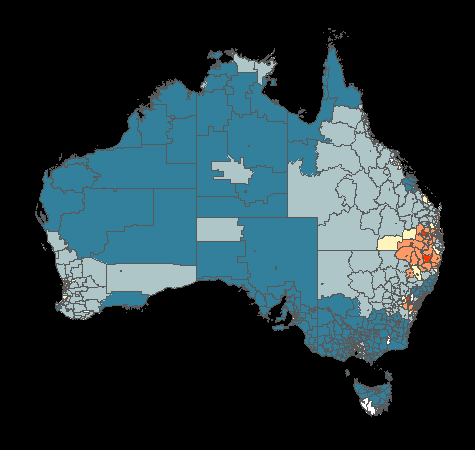
\includegraphics[width=1\linewidth,height=0.3\textheight]{paper_files/figure-latex/thyroid-choro-1} 

}

\caption{A choropleth map of thyroid incidence among females across the Statistical Areas of Australia at Level 2. Blue indicates lower than average and red indicates higher than average incidence. A cluster of high incidence is visible on the east coast.}\label{fig:thyroid-choro}
\end{figure}

The choropleth map is an effective spatial display if the size of the geographic units is relatively uniform. This is not the case for most countries. Size heterogeneity in administrative units is particularly extreme in Australia: most of the landscape of Australia is sparsely settled, with the population densely clustered into the narrow coastal strips. Fig. \ref{fig:thyroid-choro} shows the choropleth map of thyroid cancer rates in Australia. The choropleth map focuses attention on the geography, and for heterogeneously sized areas it presents a biased view of the population related distribution of the statistic {[}\protect\hyperlink{ref-CBATCC}{6}{]}. \emph{Land doesn't get cancer, people do} -- a more effective way to communicate the spatial distributions of cancer statistics is needed.

A cartogram is a general solution for better displaying a population-based statistic. It transforms the geographic map base to reflect the population in the geographic region, while preserving some aspects of the geographic location. There are several cartogram algorithms {[}\protect\hyperlink{ref-ACTUC}{7}{]}, {[}\protect\hyperlink{ref-CBATCC}{6}{]}; each involves shifting the boundaries of geographic units, using the value of the statistic to increase or decrease the area taken by the geographic unit on the map. The changes to the boundaries result in cartograms that accurately communicate population by map area for each of the geographic units but can result in losing the familiar geographic information. For Australia, the transformations warp the country so that it is no longer recognizable.

Alternative algorithms make various trade offs between familiar shapes and representation of geographic units. The non-contiguous cartogram method {[}\protect\hyperlink{ref-NAC}{8}{]} keeps the shapes of geographic units intact, and changes the size of the shape. This method disconnects areas creating empty space on the display losing the continuity of the spatial display of the statistic. The Dorling cartogram {[}\protect\hyperlink{ref-ACTUC}{7}{]} represents each unit as a circle, sized according to the value of the statistic. The neighbour relationships are mostly maintained by how the circles touch. A similar approach was pioneered by Raisz {[}\protect\hyperlink{ref-RSCW}{9}{]}, using rectangles that tile to align borders of neighbours {[}\protect\hyperlink{ref-CDWCS}{10}{]}. There have been thorough reviews of the array of methods, as suitable for cancer atlas displays {[}\protect\hyperlink{ref-review}{11}{]}, {[}\protect\hyperlink{ref-BCM}{5}{]}.

\begin{figure}

{\centering 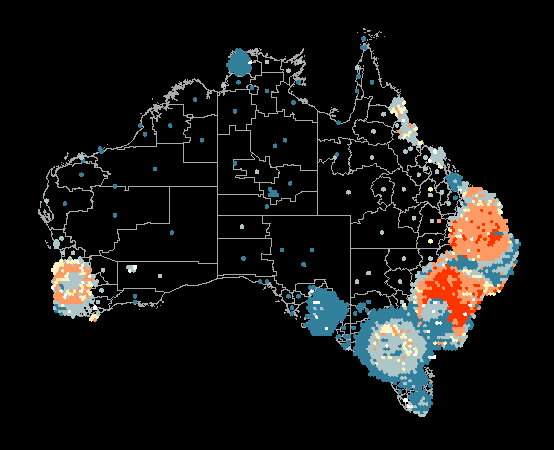
\includegraphics[width=1\linewidth,height=0.3\textheight]{paper_files/figure-latex/thyroid-hex-1} 

}

\caption{A hexagon tile map of female thyroid cancer incidence in Australia, the same data as shown in the choropleth map in Figure 1. The high incidence in several of the metropolitan regions (Brisbane, Sydney and Perth) can now be seen, along with numerous isolated spots.}\label{fig:thyroid-hex}
\end{figure}

The hexagon tile map algorithm, automatically matches spatial regions to their nearest hexagon tile, from a grid of tiles. It has the effect of spreading out the inner city areas while maintaining the spatial locations or regions in remote areas. The algorithm is available in the R package, sugarbag {[}\protect\hyperlink{ref-sugarbag}{1}{]}. Fig. \ref{fig:thyroid-hex} shows the hexagon tile map. Colour maps from substantially below average (blue) to substantially above average (red) rates. The inner city areas have expanded, making it possible to see the cancer incidence in the small, densely populated areas. Remote regions are represented by isolated hexagons, which is not ideal, but maintains the spatial location of these data values. It is of interest to know how well the spatial distribution is perceived for this display, in comparison to the choropleth.

\hypertarget{visual-inference}{%
\subsection{Visual Inference}\label{visual-inference}}

In order to assess the effectiveness of the hexagon tile map, the lineup protocol {[}\protect\hyperlink{ref-GIIV}{3}{]},{[}\protect\hyperlink{ref-BCHLLSW09}{12}{]} from visual inference procedures is employed. The approach mirrors classical statistical inference. The procedures for doing a power comparison of competing plot designed, outlined in {[}\protect\hyperlink{ref-GTPCCD}{13}{]}, are followed.

In classical statistical inference hypothesis testing is conducted by comparing the value of a test statistic on a standard reference distribution, computed assuming the null hypothesis is true. If the value is extreme, the null hypothesis is rejected, because the test statistic value is unlikely to have been so extreme if it was true. In the lineup protocol, the plot plays the role of the test statistic, and the data plot is embedded in a field of null plots. Defining the plot using a grammar of graphics {[}\protect\hyperlink{ref-ggplot2}{14}{]} makes it a functional mapping of the variables and thus, it can be considered to be a statistic. With the same data, two different plots can be considered to be competing statistics, one possibly a more powerful statistic than the other.

To do hypothesis testing with the lineup protocol requires human evaluation. The human judge is required to identify the most different plot among the field of plots. If this corresponds to the data plot -- the test statistic -- the null hypothesis is rejected. It means that the data plot is extreme relative to the reference distribution of null plots.

The null hypothesis is explicitly provided by the grammatical plot description. For example, if a histogram is the plot type being used, the null might be that the underlying distribution of the data is a Gaussian. Null data would be generated by simulating from a normal model, with the same mean and standard deviation as the data. In practice, the null hypothesis used is generic, such as \emph{there is NO structure or a pattern in the plot}, and contrasted to an alternative that there is structure.

The chance that an observer picks the data plot out of a lineup of size \(m\) plots accidentally, if the null hypothesis is true is \(1/m\). With \(K\) observers, the probability of \(k\) randomly choosing the data plot, roughly follows a binomial distribution with \(p=1/m\). Fig. \ref{fig:lineup} shows a lineup of the hexagon tile map, of size \(m=12\). Plot 3 is the data plot, and the remaining 11 are plots of null data.

\begin{figure}
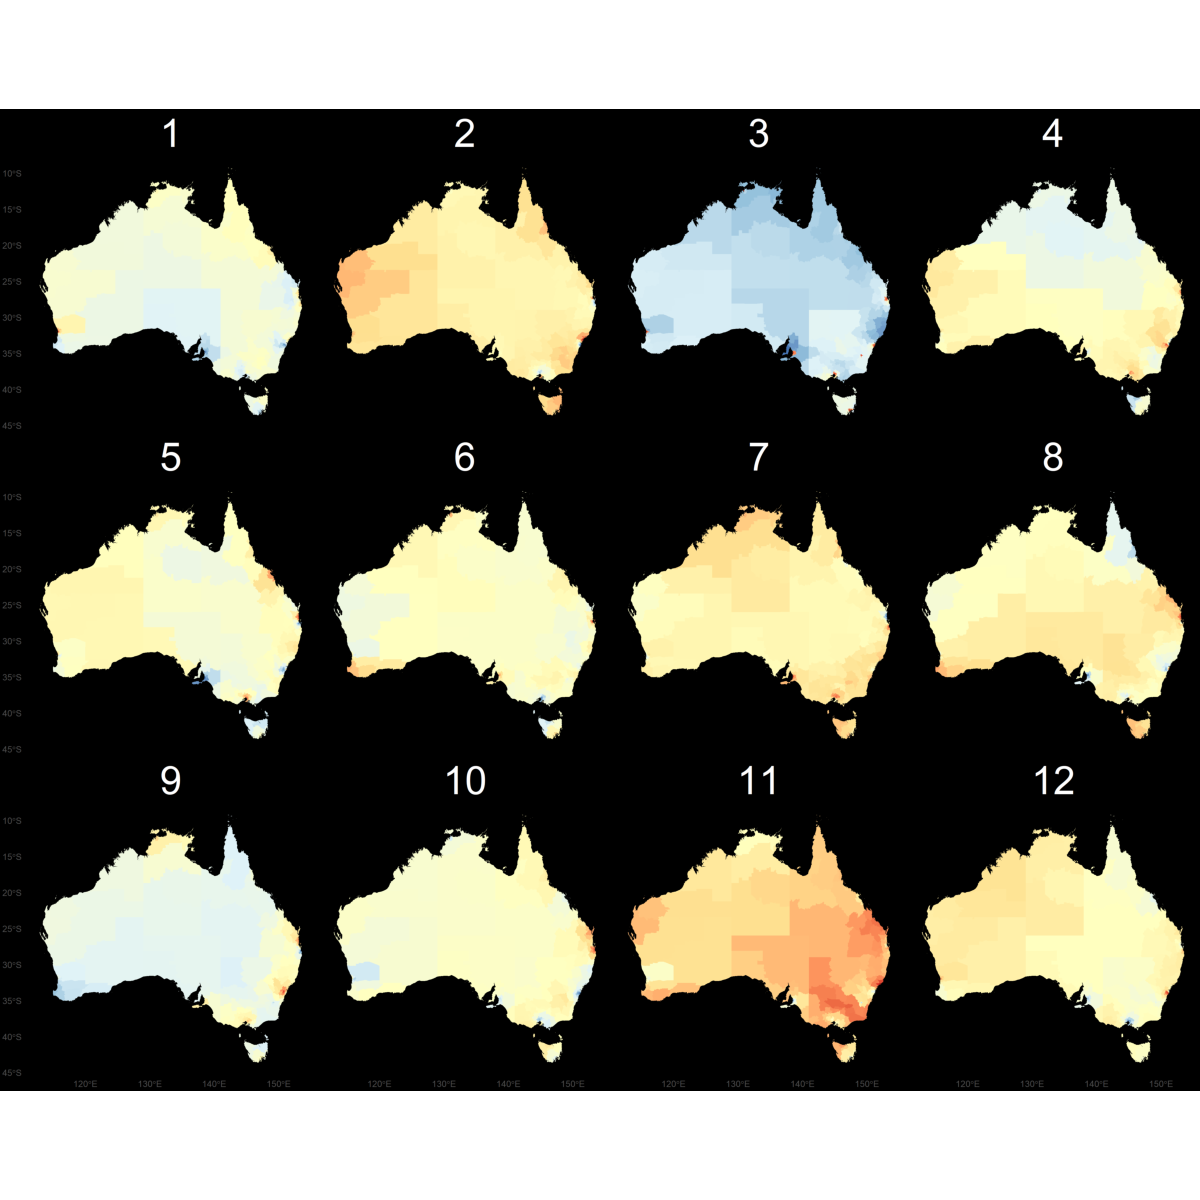
\includegraphics[width=1\linewidth]{paper_files/figure-latex/lineup-1} \caption{This lineup of twelve hexagon tile map displays contains one map with a real population related structure. The rest are null plots that contain spatial correlation between neighbours.}\label{fig:lineup}
\end{figure}

In order to determine the effectiveness of a type of display, this probability is less relevant than the overall proportion of observers who pick the data plot, \(k/K\). The power of the test statistic (data plot) is provided by this proportion. Power in a statistical sense is the ability of the statistic to \emph{produce a rejection} of the null hypothesis, if it is indeed \emph{not true}. With the same data plotted using two different displays, the display with the highest proportion of people who choose the data plot would be considered to be the most powerful statistic.

\hypertarget{methodology}{%
\section{Methodology}\label{methodology}}

This study aims to answer two key questions around the presentation of spatial distributions:

\begin{enumerate}
\def\labelenumi{\arabic{enumi}.}
\tightlist
\item
  Are spatial disease trends that impact highly populated small areas detected with higher accuracy, when viewed in a hexagon tile map?
\item
  Are people faster in detecting spatial disease trends that impact highly populated small areas when using a hexagon tile map?
\end{enumerate}

Additional considerations when completing this experimental task included the difficulty experienced by participants and the certainty they had in their decision.

Australia is used for the study, with Statistical Area 3 (SA3) {[}\protect\hyperlink{ref-abs2016}{15}{]} as the geographic units. The results should apply broadly to any other geographic area of interest.

\hypertarget{experimental-factors}{%
\subsection{Experimental factors}\label{experimental-factors}}

The primary factor in the experiment is the plot type. The secondary factor is a trend model. Three trend models were developed, one mirroring a large spatial trend for which the choropleth would be expected to do well, and two with differing level of inner city hot spots. These latter two reflect the structure seen in the thyroid cancer data (Fig. \ref{fig:thyroid}). This produces six treatment levels:

\begin{itemize}
\tightlist
\item
  Map type: \emph{Choropleth, Hexagon tile}
\item
  Trend: \emph{South-East to North-West; Locations in three population centres; Locations in multiple population centres, }
\end{itemize}

Data is generated for each of the trend models, with four replicates, and each displayed both as a choropleth and as a hexagon tile map, which yields 12 data sets, and 24 data plots. This set of displays is divided in half, providing two sets of 12 displays, Group A and Group B. Participants were randomly allocated to Group A or B. Participants saw a data set only once, either as a choropleth or as a hexagon tile map. Table \ref{fig:exp-design} summarises the design and the allocation of the displays.

\begin{figure}
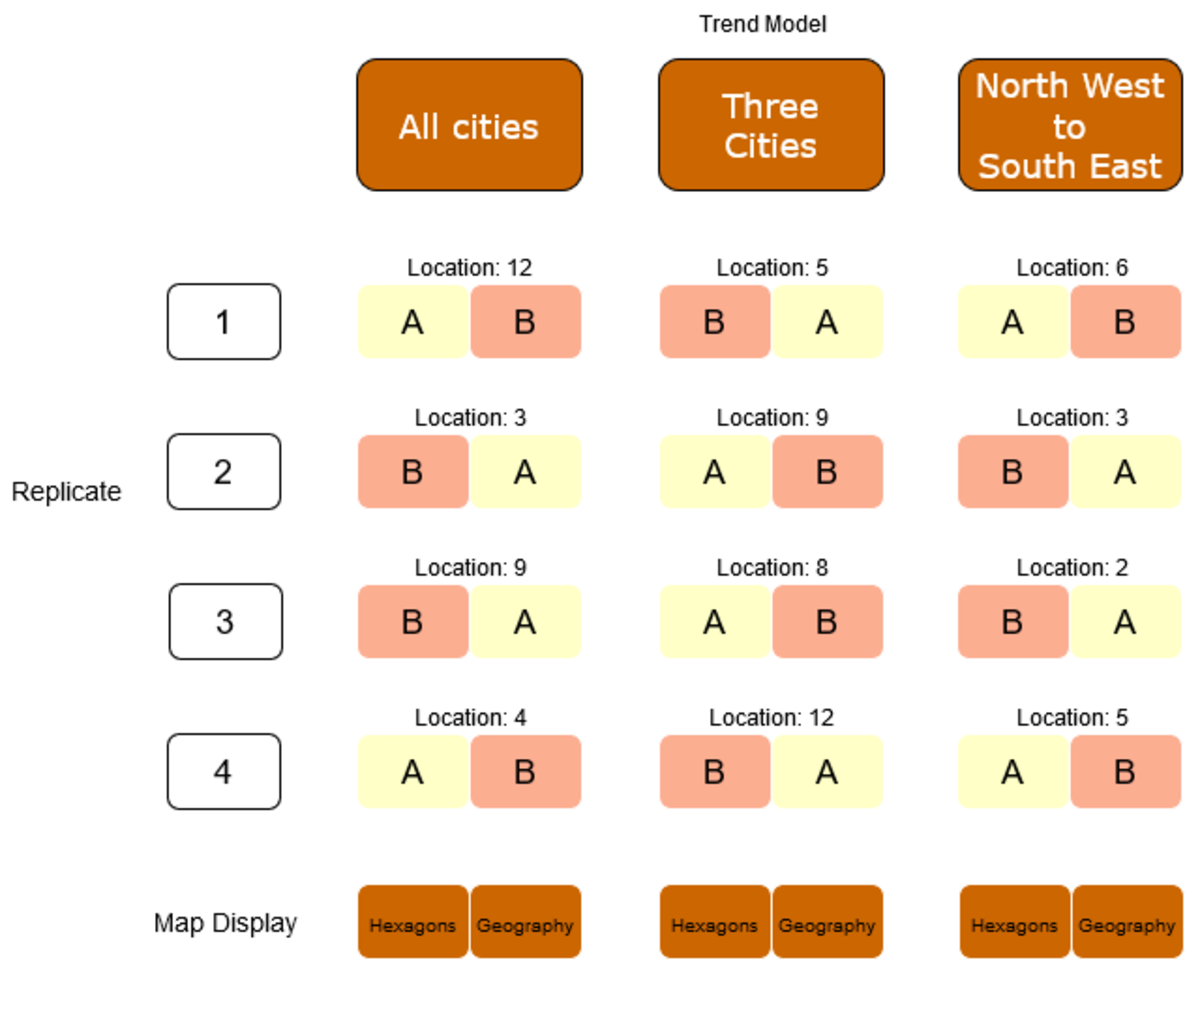
\includegraphics[width=1\linewidth]{paper_files/figure-latex/exp-design-1} \caption{The experimental design used in the visual inference study.}\label{fig:exp-design}
\end{figure}

\hypertarget{generating-null-data}{%
\subsection{Generating null data}\label{generating-null-data}}

Null data needs to be data with no (interesting) structure. In most scenarios, permutation is the main approach for generating null plots. It is used to break association between variables, while maintaining marginal distributions. This is too simple for spatial data. In spatial data, a key feature is the spatial dependence or smoothness over the landscape. To do something simple, like permute the values relative to the geographic location would produce null plots which are too chaotic, and the data plot will be recognisable for its smoothness rather than any structure of interest.

For spatial data, null data is stationary data, where the mean, variance and spatial dependence are constant over the geographic units. Stationary data is specified by a variogram model {[}\protect\hyperlink{ref-POG}{16}{]}. Simulating from a variogram model, where the spatial dependence is specified, generates the stationary spatial data used for the null plots. The parameters for the Gaussian model were sill=1, range=0.3 with the variance generated by a standard normal distribution.

The R package \texttt{gstat} {[}\protect\hyperlink{ref-gstat}{17}{]} was used to simulate 144 null sets, 12 data sets for each plot in a lineup, and 12 sets for 12 lineups.

The null model imposed by our hypothesis suggests that neighbors are related. The randomness induced when generating the null data was smoothed to mirror the practices employed by the Australian Cancer Atlas statisticians.
In these 12 sets of data, each of the 12 maps were smoothed several times to replicate the spatial autocorrelation seen in cancer data sets presented in the Australian Cancer Atlas, without implementing uncertainty via transparency.

A list of neighbors for each geographic unit was generated to use when smoothing the distributions. For each geographic unit the same spatial smoother was applied in each layer of smoothing. It kept half of the units' previous value, and derived the new half as the mean of the values of its neighbors at the previous layer of smoothing.

This smoothing allowed neighbors to be related to each other, but also allowed outliers, and showed distributions similar to the thyroid cancer distribution (Fig. \ref{fig:thyroid}).

\hypertarget{generating-lineups}{%
\subsection{Generating lineups}\label{generating-lineups}}

For each trend model, four real data displays were created by manipulating the centroid values of each of the SA3 geographic units.

The North West to South East (NW-SE) distribution was created using a linear equation of the centroid longitude and latitude values.

The All Cities trend model was created using the distance from the centroid of each geographic unit to the closest capital city in Australia, calculated when creating the hexagon tile map using the sugarbag {[}\protect\hyperlink{ref-sugarbag}{1}{]} package.
201 of the 336 SA3s were considered greater capital city areas, the values of these areas were increased to create red clusters. The amount was chosen to make clusters around the cities visible in the choropleth display even if they were not overtly noticeable.

A similar selection process was applied to the Three Cities' trend model. However, for each of the four replicates for the Three Cities trend, a random sample of capital cities was taken from Sydney, Brisbane, Melbourne, Adelaide, Perth, and Hobart. Only values of the areas nearest to the three cities were increased to create clusters.

One of the lineup locations was chosen to embed the real trend model map, in each of the four replicates, for the three trend models.
The location was chosen from a sub sample of the 12 possible locations. The chance of reptition using resampling was introduced to prevent participants from inducing the location by elimination, the locations 1, 7, 10 and 11 were not used.

As seen in Fig \ref{fig:exp-design}, the choropleth and hexagon display used the same location for the real data display of the trend model was added to the spatially correlated null values for each lineup.
Each set of lineup data was used to produce a choropleth map lineup and hexagon tile map lineup. These matched pairs were split between Group A and Group B according to the 2 x 3 factor experimental design depicted in \ref{fig:exp-design}.

For each of the 144 individual maps, the values for each geographic area were rescaled to create a similar color scale from deep blue to dark red within each map.
This meant at least one geographic unit was coloured dark blue, and at least one was red, in every map display of every lineup.

For the geographic NW-SE distribution, this resulted in the smallest values of the trend model (blue) occurring in Western Australia, the North West of Australia, and the largest values of the trend model (red) occurring in the South East. This resulted in Tasmania being colored completely red.

For the population related displays, the clusters in the cities appeared more red than the rest of Australia.

\hypertarget{analysis}{%
\subsection{Analysis}\label{analysis}}

\hypertarget{data-cleaning}{%
\subsubsection{Data Cleaning}\label{data-cleaning}}

The first step in the data cleaning process involved checking that survey responses collected for each participants were only included once in the data set.
The data cleaning process also involved filtering out participants' who did not provide at least three unique choices when considering each of the twelve lineups. These participants achieved a detection rate of 0. If participants had made various plot choices for the 12 displays they saw they were still included in the dataset.

\hypertarget{descriptive-statistics}{%
\subsubsection{Descriptive statistics}\label{descriptive-statistics}}

Basic descriptive statistics were used to contrast the detection rate for the two types of displays. Comparison was also made across the trend models, contrasting the mean and standard detection rate for each group, who had seen the different map display type for each replicate.

Side-by-side dot plots were made of accuracy (efficiency) against map type, faceted by trend model type.

Similar plots were made of the feedback and demographic variables - reason for choice, reported difficulty, gender, age, education, having lived in Australia - against the design variables.

Plots will be made in R {[}\protect\hyperlink{ref-RCore}{18}{]}, with the \texttt{ggplot2} package {[}\protect\hyperlink{ref-ggplot2}{14}{]}.

\hypertarget{modelling}{%
\subsubsection{Modelling}\label{modelling}}

The likelihood of detecting the data plot in the lineup can be modelled using a linear mixed effects model.
The R {[}\protect\hyperlink{ref-RCore}{18}{]} \texttt{glmer()} function in the \texttt{lme4} {[}\protect\hyperlink{ref-lme4}{19}{]} package implements generalised linear mixed effect models. The model used includes the two main effects map type and trend model, which gives the fixed effects model to be:

\[\widehat{y_{ij}} = \mu + \tau_i + \delta_j + (\tau\delta)_{ij} + \epsilon_{i,j}, ~~~ i=1,2; ~j=1,2,3\]

where \(y_{ij} = 0, 1\) is the logg odds for whether the subject detected the data plot, \(\mu\) is the overall mean, \(\tau_i, i=1,2\) is the map type effect, \(\delta_j\) is the trend model effect. We are allowing for an interaction between map type and trend model as the response is binary, so a logistic model was used. As each participant provides results from 12 lineups, this model can account for each individual participants' abilities as it includes a subject-specific random intercept.

The model specifies a logistic link, this means the predicted values from the \texttt{glmer} model should be back-transformed to fit between 0 and 1. The predictions \(\widehat{p}(\eta)\) are transformed to be probabilities between 0 and 1 with the link specified below:

\[\widehat{p}(\eta) = \frac{e^{\eta}}{1 + e^{\eta}}\] \label{eq:transform}
\[\eta = f(\tau_i,\delta_j)\]

\hypertarget{web-application-to-collect-responses}{%
\subsection{Web application to collect responses}\label{web-application-to-collect-responses}}

The taipan {[}\protect\hyperlink{ref-taipan}{20}{]} package for R was used to create the survey web application.
This structure was altered to collect responses regarding participants demographics and their survey responses.
The survey app contained three tabs. Participants were first asked for their demographics their Figure Eight contributor ID, and their consent to the responses being used for analysis. The demographics collected included participants' preferred pronoun, the highest level of education achieved, their age range and whether they had lived in Australia.

After submitting these responses, the survey application switched to the tab of lineups and associated questions. This allowed participants to easily move through the twelve displays and provide their choice, reason for their choice, and level of certainty.

When participants completed the twelve evaluations the survey application triggered a data analysis script. This created a data set with one row per evaluation. Containing the responses to the three questions. The script also added the title of the image, which indicated the type of map display, the type of distribution hidden in the lineup, and the location of the data plot. It also calculated the time taken by participant to view each lineup.

Each participant used the internet to access the survey.
The data transfer from the web application to the data set took place using a secure link to the googlesheet used to store results. The application connected to the googlesheet using the googlesheets {[}\protect\hyperlink{ref-sheets}{21}{]} R package when participants opened the application, and interacted again when participants chose to submit the survey. At this time it added the participant's responses to the twelve lineup displays as twelve rows of data in the googlesheet.

\hypertarget{participants}{%
\subsection{Participants}\label{participants}}

Participants were recruited from the Figure Eight crowdsourcing platform {[}\protect\hyperlink{ref-figeight}{22}{]} to evaluate lineups.
The lineup protocol expects that the participants are uninvolved judges with no prior knowledge of the data, to avoid inadvertently affecting results. Potential participants needed to have achieved level 2 or level 3 from prior work on the platform. All participants were at least 18 years old.

Participants were allocated to either group A or group B when they proceeded to the survey web application. There were 92 participants involved in the study. All participants read introductory materials, and were trained using three test displays, to orient them to the evaluation task. All participants who completed the task were compensated \$AUD5 for their time, via the Figure Eight payment system.

A pilot study was conducted in the working group of the Econometrics and Business Statistics Department of Monash University. This allowed us to estimate the effect size, and thus decide on number of participants to collect responses from.

\hypertarget{demographic-data-collection}{%
\subsection{Demographic data collection}\label{demographic-data-collection}}

Each participant answered demographic questions and provided consent before evaluating the lineups.

Demographics were collected regarding the study participants:

\begin{itemize}
\tightlist
\item
  Gender (female / male / other),
\item
  Education level achieved (high school / bachelors / masters / doctorate / other),
\item
  Age range (18-24 / 25-34 / 35-44 / 45-54 / 55+ / other)
\item
  Lived at least for one year in Australia (Yes / No )
\end{itemize}

Participants then moved to the evaluation phase.
The set of images differed for Group A and Group B.
After being allocated to a group, each individual was shown the 12 displays in randomised order.

Three questions were asked regarding each display:

\begin{itemize}
\tightlist
\item
  Plot choice
\item
  Reason
\item
  Difficulty
\end{itemize}

After completing the 12 evaluations, the participants were asked to submit their responses.

\hypertarget{results}{%
\section{Results}\label{results}}

Responses from 92 participants were collected. Five participants did not provide more than three unique choices for the twelve lineups, and their data was removed. Set A was evaluated by 42 participants, and 53 evaluated set B. This resulted in 1104 evaluations, corresponding to 92 subjects, each evaluating 12 lineups, that were analysed on accuracy and speed. The certainty and reasons of subjects in their answers is also examined.

\hypertarget{participant-demographics}{%
\subsection{Participant demographics}\label{participant-demographics}}

Of the 92 participants, 67 were male, and 25 female. Most participants (56) had a Bachelors degree, 13 had a Masters degree, and the remaining 23 had high school diplomas.

\hypertarget{accuracy}{%
\subsection{Accuracy}\label{accuracy}}

Fig. \ref{fig:detect-compare} displays the average detection rates for the two types of plot separately for each trend model. Each trend model was tested using four repetitions, evaluations on the same data set were seen as either choropleths or hexagon tile maps by each group as specified in Table. \ref{fig:exp-design}; the detection rates for each display are connected by a line segment. The Three Cities and All Cities trend models shown in the hexagon tile map allowed viewers to detect the data plot substantially more often than the choropleth counterparts. One replicate for the All Cities group had similar detection rates for both plot types, the rate of detection using the choropleth map was much higher than other replicates. Surprisingly, participants could also detect the gradual spatial trend in the NW-SE group from the hexagon tile map. We expected that the choropleth map would be superior for the type of spatial pattern, but the data suggests the hexagon tile map performs slightly better, or equally as well.

\begin{figure}
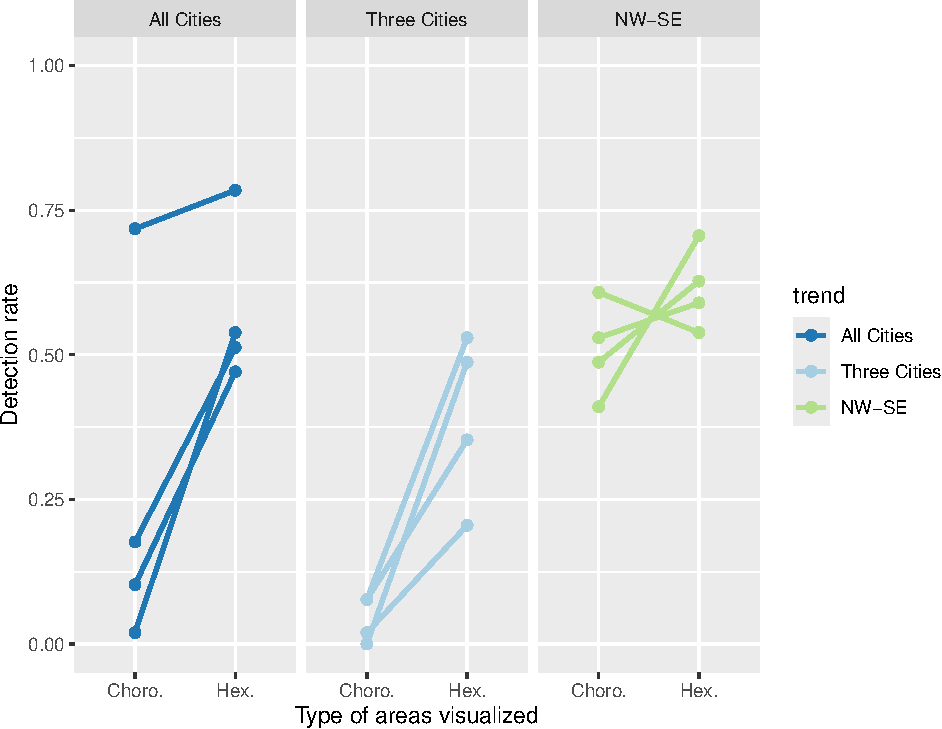
\includegraphics[width=1\linewidth]{paper_files/figure-latex/detect-compare-1} \caption{The detection rates achieved by participants are contrasted when viewing the four replicates of the three trend models. Each point shows the probability of detection for the lineup display, the facets separate the trend models hidden in the lineup. The points for the same data set shown in a choroleth or hexagon tile map display are linked to show the difference in the detection rate.}\label{fig:detect-compare}
\end{figure}

Table. \ref{tab:desc-stats} shows the means and standard deviations of the detection rate for each type of plot and each trend model. This also gives the standard deviations, the smallest standard deviation for all sets of replicates was the Three Cities trend model shown in a Choropleth display. This group of displays had a very small detection rate of 0.04. The mean detection rate for the Three Cities trend model shown as choropleth map lineups was also the smallest at 0.40.
The North-West to South-East (NW-SE) trend model unexpectedly had a higher mean detection rate for the hexagon tile map displays, but the difference in the means of detection rate was only 0.10.

\begin{table}

\caption{\label{tab:desc-stats}The mean and standard deviation of the rate of detection for each trend model, calculated for the choropleth and hexagon tile map displays.}
\centering
\begin{tabular}[t]{lccc}
\toprule
Type & NW-SE & Three Cities & All Cities\\
\midrule
Choro. & 0.52 & 0.04 & 0.23\\
 & (0.50) & (0.19) & (0.42)\\
\addlinespace
Hex. & 0.62 & 0.40 & 0.58\\
 & (0.49) & (0.49) & (0.49)\\
\bottomrule
\end{tabular}
\end{table}

Table. \ref{tab:detect-glmer1} presents a summary of the generalised linear mixed effects model, testing the effect of plot type and trend model on the detection rate. The results support the summary from Fig. \ref{fig:detect-compare} and all parameters are statistically significant despite the large standard deviations observed in Table. \ref{tab:desc-stats}. Overall, the hexagon tile map performs marginally better than the choropleth for all trend models, which is a pleasant surprise. Allowing for the interaction effect, the difference in detection rate decreases for population related displays for a choropleth map lineup, but increases for a hexagon tile map display.
The log odds of detection show in Table. \ref{tab:detect-glmer1} can be back transformed after taking the sum of all terms for the trend and type of display that are of interest.
For the NW-SE distribution, the predicted detection rate for the hexagon tile map display increases the predicted probability of detection to 0.63 from 0.52 for choropleths, this is almost exactly the difference seen in the table of means and is significant only at the 0.05 level.

When a choropleth map display is used, the predicted detection rate for the Three Cities trend, 0.03; this is extremely low, especially compared to the NW-SE trend of 0.52.
When the All Cities trend is presented in a choropleth display the predicted probability of detection is 0.22.
The hexagon tile map has a substantially high detection rate for the display of a Three Cities trend 0.39 and All Cities trend 0.59.

\begin{table}

\caption{\label{tab:detect-glmer1}The model output for the generalised linear mixed effect model for detection rate. This model considers the type of display, the trend model hidden in the data plot, and accounts for contributor performance.}
\centering
\begin{tabular}[t]{rrlrr}
\toprule
Term & Est. & Sig. & Std. Error & P val\\
\midrule
Intercept & -1.27 & $^{***}$ & 0.19 & 0.00\\
Hex. & 1.63 & $^{***}$ & 0.24 & 0.00\\
\addlinespace
Three Cities & -2.07 & $^{***}$ & 0.43 & 0.00\\
All Cities & 1.34 & $^{***}$ & 0.24 & 0.00\\
\addlinespace
Hex:Three Cities & 1.28 & $^{**}$ & 0.48 & 0.01\\
Hex:All Cities & -1.16 & $^{***}$ & 0.33 & 0.00\\
\bottomrule
\end{tabular}
\end{table}

\hypertarget{speed}{%
\subsection{Speed}\label{speed}}

Fig. \ref{fig:beeswarm} shows horizontally jittered dot plots to contrast the time taken by participants to evaluate each lineup when viewing each type of display. The time are also separated by trend model and whether the data plot was detected or not detected. The time taken to complete an evaluation ranged from milliseconds to 60 seconds. The average time taken for type of display is shown as a large colored dot on each plot. when considering the heights of the green and orange dots, there is little difference in the average time taken to read a choropleth or hexagon tile map. Comparing the same colored dot across each trend model row, there is a slight increase in the time taken to correctly detected the data plot in the hexagon tile map lineup, but little difference in evaluation time for the choropleth display. However, there were substantially less correct detections for choropleth lineups for the Three cities and All Cities trends.

\begin{figure}
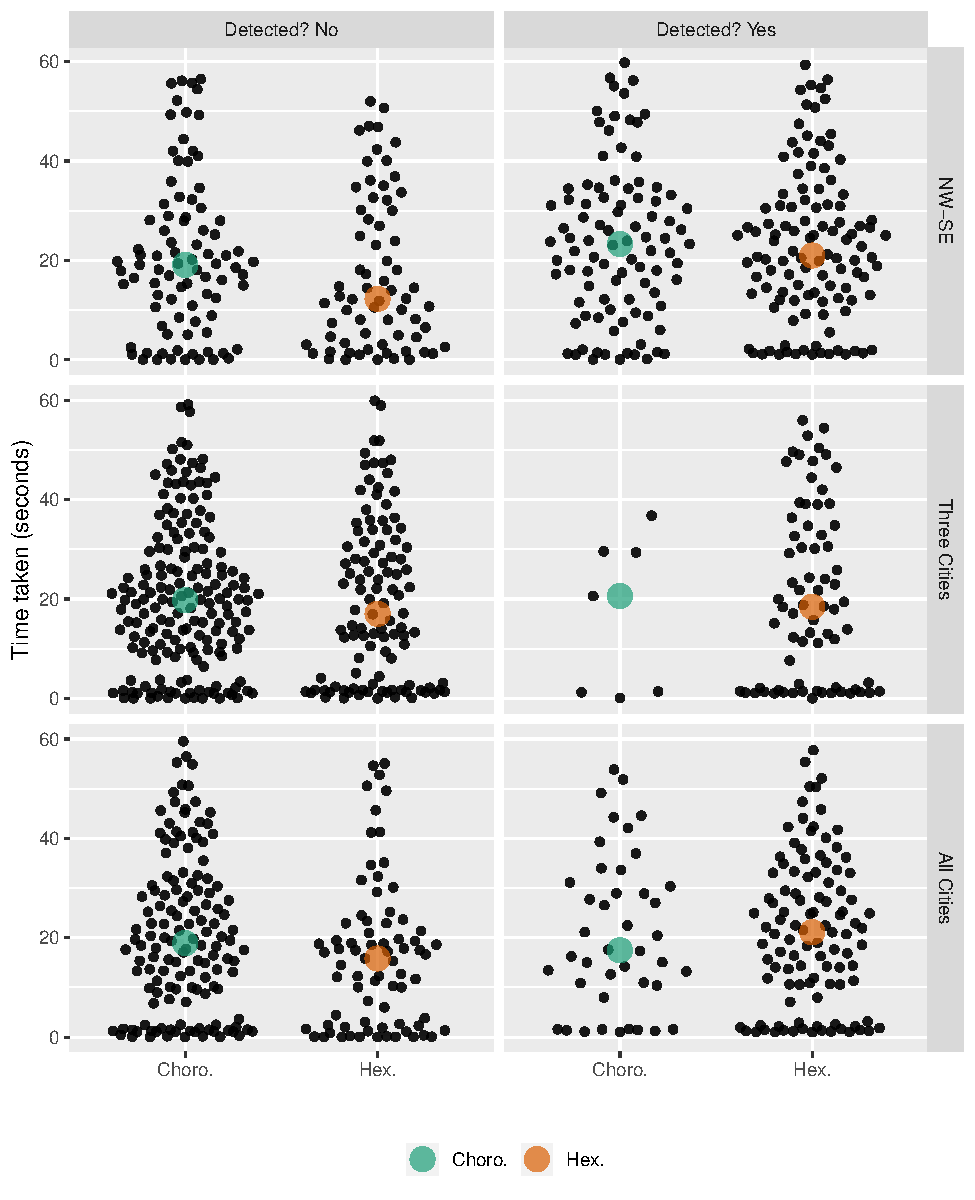
\includegraphics[width=1\linewidth]{paper_files/figure-latex/beeswarm-1} \caption{The distribution of the time taken (seconds) to submit a response for each combination of trend, whether the data plot was detected, and type of display, shown using horizontally jittered dotplots. The colored point indicates average time taken for each plot type. Although some participants take just a few seconds per evaluation, and some take as much as mcuh as 60 seconds, but there is very little difference in time taken between plot types.}\label{fig:beeswarm}
\end{figure}

\hypertarget{certainty}{%
\subsection{Certainty}\label{certainty}}

Participants provided their level of certainty regarding their choice using a five point scale.
Unlike the accuracy and speed of responses that were derived during the data processing phase, this was a subjective
assessment by the participant prompted by the question: `How certain are you about your choice?'.
Fig. \ref{fig:certainty} shows the amount of times participants provided each level of certainty. This was separated for each combination of trend models and display type, and colored depending on whether a participant correctly detected the data plot in the lineup.
Participants often chose 4 or 5 when viewing the population related trends in the choropelth display, even though they were often incorrect when viewing an All Cities trend and overwhelmingly incorrect for the Three Cities trend. This shows overconfidence in their detection ability when using a choropleth map display. Participants were less likely to be certain when their choice was incorrect and they were viewing a hexagon tile map.
For each trend model, participants were more likely to doubt their choice and choose 1 or 2 in the hexagon tile map displays, even though many had made the correct choice.

\begin{figure}
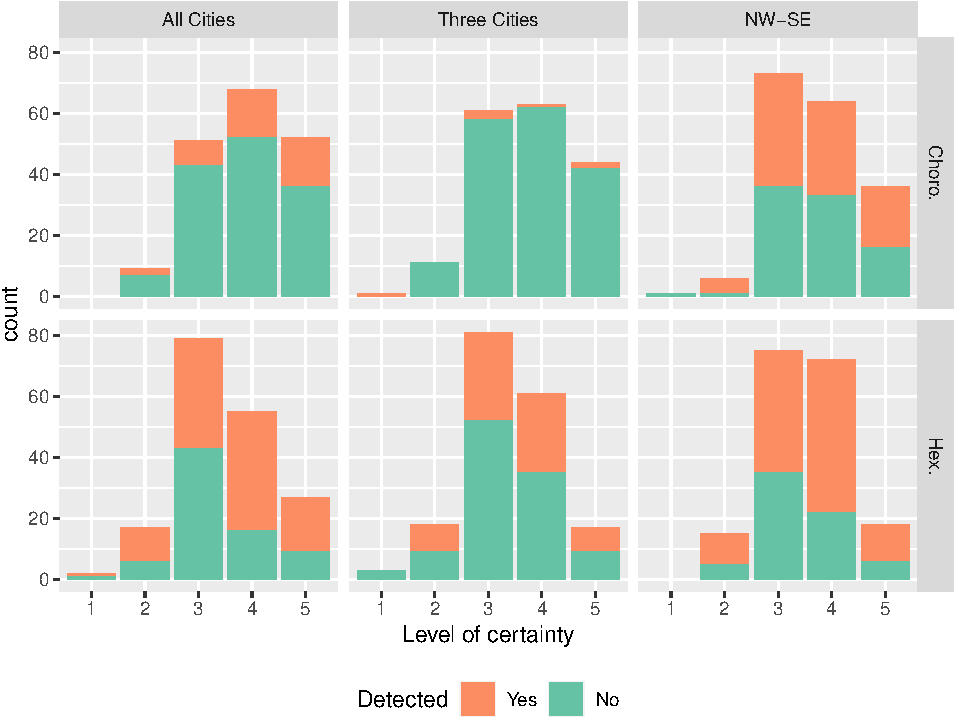
\includegraphics[width=1\linewidth]{paper_files/figure-latex/certainty-1} \caption{The amount of times each level of certainty was chosen by participants when viewing hexagon tile map or choropleth displays. Participants were more likely to choose a high certainty when considering a Choropleth map. The mid value of 3 was the default certainty, it was chosen most for the Hexagon tile map displays.}\label{fig:certainty}
\end{figure}

\hypertarget{reason}{%
\subsection{Reason}\label{reason}}

Participants were asked why they had made their plot choice and were able to select from a set of suggested reasons.
``Color trend across the areas'' was the most common selection for NW-SE trend displays.

The reasons chosen by participants from the list provided to them varied more when viewing choropleth displays than the hexagon tile map.
The hexagon tile map displays resulted in ``Clusters of color'' as the most common choice made by participants.

The choice ``None of these reasons'' was used as the default value to minimise noise from participants who did not select a response.

\begin{table}

\caption{\label{tab:reason}The amount of participants that selected each reason for their choice of plot when looking at each trend model shown in Choropleth and Hexagon Tile maps. The facets show whether or not the choice was correct.}
\centering
\begin{tabular}[t]{llll}
\toprule
Trend & Detected & Choro. & Hex.\\
\midrule
 & No & trend & clusters\\
\cmidrule{2-4}
\multirow{-2}{*}{\raggedright\arraybackslash All Cities} & Yes & clusters, consistent & clusters\\
\cmidrule{1-4}
 & No & trend & clusters\\
\cmidrule{2-4}
\multirow{-2}{*}{\raggedright\arraybackslash Three Cities} & Yes & consistent & clusters\\
\cmidrule{1-4}
 & No & trend & clusters\\
\cmidrule{2-4}
\multirow{-2}{*}{\raggedright\arraybackslash NW-SE} & Yes & trend & clusters\\
\bottomrule
\end{tabular}
\end{table}

\hypertarget{discussion}{%
\section{Discussion}\label{discussion}}

The intention of this study was to contrast the use of the choropleth map and the hexagon tile map.
The visual inference lineup protocol was employed to contrast the effectiveness of the displays.
The results have shown that overall the use of the hexagon tile map display allows participants to find the data plot in the lineup more often.
Using the visual inference protocol this result can be extended to show that it is a valid alternative display to communicate spatial distributions of population related data.

We expected that the choropleth map would be superior for communicating the spatial pattern of geographic distributions. The data suggest that the participants perform slightly better or equally as well for each replicate in each trend model across the two displays. Table II shows that the difference in the mean detection rate for the two trend models was 0.10.

The differences seen in the \ref{fig:detect-compare} plot and Table. \ref{tab:desc-stats} are reflected in the model results. Surprisingly the difference for the geographic distribution was significant at the 0.05 level.
It also showed that the hexagon tile map display performs marginally better than the choropleth for all trend models. Unexpectedly the detection rate suffers when using a choropleth map to display population related distributions.

While the significance of the difference in detection was the key focus of this experiment, the secondary focus was the time taken by participants. it was expected that the participants may take longer to consider the hexagon tile map distribution but would be able to detect the data plot in the lineup.
The bimodal distributions seen in Fig. \ref{fig:beeswarm} showed very little difference in the mean evaluation times. As the maximum time of all of the distributions approached 60 seconds it cannot be said that the participants' took longer to evaluate the hexagon tile map displays.

The responses to the questions asked of participants included the reason for their choice and the certainty around their choice.
Fig. \ref{tab:reason} shows high levels of certainty of 4 and 5 were chosen by participants when looking at the population distributions in a choropleth map display show that they were over confident when attempting to find the real data plot in the choropleth map displays. Participants performed better on the NW-SE distribution shown in the choropleth display and were reasonably confident about their decisions.
The high levels of the mid range value of 3 could indicate that the participant did not want to provide a response, as this was the default value. Those who chose level 4 or 5 were equally likely to be correct for the three cities lineups, but more likely to be correct than incorrect for the other two trend models.

The color scaling applied in Three cities and All cities displays resulted in the rural areas of the real data plot appearing more blue or yellow than the other plots in the lineups.
Due to the consistent coloring of rural areas in a choropleth display, the choice ``All areas have similar colors'' was most common reason for a participants choice. The All Cities displays colored the inner-city areas of all capital cities more red, this was observable to participants and explains the equal choice of the city clusters or rural color consistency.
Choosing ``Clusters of colour'' was expected when participants viewed the Hexagon tile map display of the All Cities and Three Cities distributions. It was unexpected that it was also the most common reason for the NW-SE hexagon tile map displays.
Due to the spatial covariance introduced in the smoothing, groups of similarly colored hexagons were present in all of the hexagon tile map displays. All Cities and Three Cities distributions of real data trends had distinctly different patterns or red inner-city areas, while some of the plots in each lineup may have shared similar features.

\hypertarget{conclusion}{%
\section{Conclusion}\label{conclusion}}

The choropleth map display and the tessellated hexagon tile map have been contrasted using the lineup protocol. The hexagon tile map was significantly more effective for spotting a real population related data trend model hidden in a lineup.

The hexagon tile map display should be considered as an alternative visualization method when communicating distributions that relate to the population across a set of geographic units. As an additional display to the familiar choropleth map, cancer atlas products may benefit from the opportunity to allow exploration via an alternative display. The spatial distributions used to test these displays were inspired by the real spatially smoothed estimates of the cancer burden on Australian communities. However, this technique may be extended to other population related distributions, such as other diseases.

The increasing population densities of capital cities despite large land area exacerbates the difference in the smallest and largest communities.
The population density structure of Australia can be considered similar to that of Canada, New Zealand and many other countries. Therefore, this display is not only relevant to Australia, but all nations or population distributions that experience densely populated cities separated by vast rural expanses.

\hypertarget{acknowledgment}{%
\section{Acknowledgment}\label{acknowledgment}}

The authors would like to thank the Australian Cancer Atlas team for discussions regarding alternative spatial visualizations, and Professor Kerrie Mengersen and Dr Earl Duncan for regular meetings filled with suggestions and comments. Mitchell O'Hara-Wild was a co-developer of the taipan {[}\protect\hyperlink{ref-taipan}{20}{]} R package for image tagging, used as the base for the web app constructed to collect participant evaluations of lineups. We are thankful for the NUMBATs (Non-Uniform Monash Business Analytics Team) for participating in the pilot study that helped to assess the experimental design and determine an appropriate sample size for the study.

The source code to produce this document can be found on \href{https://github.com/srkobakian/experiment/paper}{GitHub}.
Supplementary materials have been included to discuss the survey procedures and the lineups that were used.
The full set of images can be found here, too.

The supplementary material contains:

\begin{itemize}
\tightlist
\item
  Additional analysis of the experimental results
\item
  Survey procedure including training materials for the participants
\item
  24 lineups as images, that were used in the experiment
\item
  12 data sets used to construct the lineups
\end{itemize}

The analysis of the work was completed in R {[}\protect\hyperlink{ref-RCore}{18}{]} with the use of the following packages:

\begin{itemize}
\tightlist
\item
  For document creation: rmarkdown {[}\protect\hyperlink{ref-rmarkdown}{23}{]}, rticles {[}\protect\hyperlink{ref-rticles}{24}{]}, knitr {[}\protect\hyperlink{ref-knitr}{25}{]}.
\item
  For lineup creation and data analysis: tidyverse {[}\protect\hyperlink{ref-tidyverse}{26}{]}, nullabor {[}\protect\hyperlink{ref-nullabor}{27}{]}, ggthemes {[}\protect\hyperlink{ref-ggthemes}{28}{]}, RColorBrewer {[}\protect\hyperlink{ref-RColorBrewer}{29}{]}.
\item
  For image displays: cowplot {[}\protect\hyperlink{ref-cowplot}{30}{]}, png {[}\protect\hyperlink{ref-png}{31}{]}, grid {[}\protect\hyperlink{ref-grid}{32}{]}.
\item
  For modelling and presentation of models: gstat {[}\protect\hyperlink{ref-gstat}{17}{]}, lme4 {[}\protect\hyperlink{ref-lme4}{19}{]}, kableExtra {[}\protect\hyperlink{ref-kableExtra}{33}{]}.
\end{itemize}

Ethics approval for the online survey was granted by QUT's Ethics Committee (Ethics Application Number: 1900000991). All applicants provided informed consent in line with QUT regulations prior to participating in this research.

\hypertarget{references}{%
\section*{References}\label{references}}
\addcontentsline{toc}{section}{References}

\hypertarget{refs}{}
\begin{CSLReferences}{0}{0}
\leavevmode\vadjust pre{\hypertarget{ref-sugarbag}{}}%
\CSLLeftMargin{1. }%
\CSLRightInline{Kobakian S, Cook D (2019) Sugarbag: Create tessellated hexagon maps. }

\leavevmode\vadjust pre{\hypertarget{ref-atlas}{}}%
\CSLLeftMargin{2. }%
\CSLRightInline{Cancer Council Queensland {Australian Cancer Atlas}, publisher = {Queensland University of Technology, Cooperative Research Centre for Spatial Information}, issue = {Version 09}, url={https://atlas.cancer.org.au}, year = {2018}, accessed = {Jan 12 2020}. }

\leavevmode\vadjust pre{\hypertarget{ref-GIIV}{}}%
\CSLLeftMargin{3. }%
\CSLRightInline{Wickham H, Cook D, Hofmann H, Buja A (2010) Graphical inference for infovis. IEEE Transactions on Visualization and Computer Graphics (Proc InfoVis '10) 16:973--979}

\leavevmode\vadjust pre{\hypertarget{ref-EI}{}}%
\CSLLeftMargin{4. }%
\CSLRightInline{Tufte ER (1990) {Envisioning Information}. Graphics Press}

\leavevmode\vadjust pre{\hypertarget{ref-BCM}{}}%
\CSLLeftMargin{5. }%
\CSLRightInline{Skowronnek A (2016) \href{https://alsino.io/static/papers/BeyondChoropleths_AlsinoSkowronnek.pdf}{{Beyond Choropleth Maps -- A Review of Techniques to Visualize Quantitative Areal Geodata}}. {Infovis Reading Group WS 2015/16} }

\leavevmode\vadjust pre{\hypertarget{ref-CBATCC}{}}%
\CSLLeftMargin{6. }%
\CSLRightInline{Kocmoud C, House D (1998) {A Constraint-based Approach to Constructing Continuous Cartograms}. In: Proc. Symp. Spatial data handling. pp 236--246}

\leavevmode\vadjust pre{\hypertarget{ref-ACTUC}{}}%
\CSLLeftMargin{7. }%
\CSLRightInline{Dorling D (2011) \href{https://doi.org/10.1002/9780470979587.ch33}{{Area Cartograms: Their Use and Creation}}. In: Concepts and techniques in modern geography (CATMOG). University of East Anglia: Environmental Publications, pp 252--260}

\leavevmode\vadjust pre{\hypertarget{ref-NAC}{}}%
\CSLLeftMargin{8. }%
\CSLRightInline{Olson JM (1976) \href{https://doi.org/10.1111/j.0033-0124.1976.00371.x}{{Noncontiguous Area Cartograms}}. The Professional Geographer 28:371--380}

\leavevmode\vadjust pre{\hypertarget{ref-RSCW}{}}%
\CSLLeftMargin{9. }%
\CSLRightInline{Raisz E (1963) \href{https://doi.org/10.1080/00221343608987880}{{Rectangular Statistical Cartograms of the World}}. Journal of Geography 35:8--10}

\leavevmode\vadjust pre{\hypertarget{ref-CDWCS}{}}%
\CSLLeftMargin{10. }%
\CSLRightInline{Monmonier M (2005) \href{https://doi.org/10.1191/0309132505ph540pr}{{Cartography: Distortions, World-views and Creative Solutions}}. Progress in Human Geography 29:217--224}

\leavevmode\vadjust pre{\hypertarget{ref-review}{}}%
\CSLLeftMargin{11. }%
\CSLRightInline{Kobakian S, Cook D, Roberts J (2020) \href{https://ace.amegroups.com/article/view/6040}{Mapping cancer: The potential of cartograms and alternative map displays}. Annals of Cancer Epidemiology 4:}

\leavevmode\vadjust pre{\hypertarget{ref-BCHLLSW09}{}}%
\CSLLeftMargin{12. }%
\CSLRightInline{Buja A, Cook D, Hofmann H, Lawrence M, Lee E-K, Swayne DF, Wickham H (2009) \href{https://doi.org/10.1098/rsta.2009.0120}{Statistical inference for exploratory data analysis and model diagnostics}. Philosophical Transactions of the Royal Society, A (Invited) 367:4361--4383}

\leavevmode\vadjust pre{\hypertarget{ref-GTPCCD}{}}%
\CSLLeftMargin{13. }%
\CSLRightInline{Hofmann H, Follett L, Majumder M, Cook D (2012) Graphical tests for power comparison of competing designs. IEEE Transactions on Visualization and Computer Graphics 18:2441--2448}

\leavevmode\vadjust pre{\hypertarget{ref-ggplot2}{}}%
\CSLLeftMargin{14. }%
\CSLRightInline{Wickham H (2009) \href{http://had.co.nz/ggplot2/book}{ggplot2: Elegant graphics for data analysis}. Springer New York}

\leavevmode\vadjust pre{\hypertarget{ref-abs2016}{}}%
\CSLLeftMargin{15. }%
\CSLRightInline{Australian Bureau of Statistics (2018) \href{https://www.abs.gov.au/statistics/statistical-geography/australian-statistical-geography-standard-asgs}{{Australian Statistical Geography Standard (ASGS)}}. }

\leavevmode\vadjust pre{\hypertarget{ref-POG}{}}%
\CSLLeftMargin{16. }%
\CSLRightInline{Matheron G (1963) \href{http://dx.doi.org/10.2113/gsecongeo.58.8.1246}{Principles of geostatistics}. Economic Geology 58:1246--1266}

\leavevmode\vadjust pre{\hypertarget{ref-gstat}{}}%
\CSLLeftMargin{17. }%
\CSLRightInline{Gräler B, Pebesma E, Heuvelink G (2016) \href{https://journal.r-project.org/archive/2016/RJ-2016-014/index.html}{Spatio-temporal interpolation using gstat}. The R Journal 8:204--218}

\leavevmode\vadjust pre{\hypertarget{ref-RCore}{}}%
\CSLLeftMargin{18. }%
\CSLRightInline{R Core Team (2019) \href{https://www.R-project.org/}{R: A language and environment for statistical computing}. R Foundation for Statistical Computing, Vienna, Austria}

\leavevmode\vadjust pre{\hypertarget{ref-lme4}{}}%
\CSLLeftMargin{19. }%
\CSLRightInline{Bates D, Mächler M, Bolker B, Walker S (2015) \href{https://doi.org/10.18637/jss.v067.i01}{Fitting linear mixed-effects models using {lme4}}. Journal of Statistical Software 67:1--48}

\leavevmode\vadjust pre{\hypertarget{ref-taipan}{}}%
\CSLLeftMargin{20. }%
\CSLRightInline{Kobakian S, O'Hara-Wild M (2018) \href{https://CRAN.R-project.org/package=taipan}{Taipan: Tool for annotating images in preparation for analysis}. }

\leavevmode\vadjust pre{\hypertarget{ref-sheets}{}}%
\CSLLeftMargin{21. }%
\CSLRightInline{Bryan J, Zhao J (2018) \href{https://CRAN.R-project.org/package=googlesheets}{Googlesheets: Manage google spreadsheets from r}. }

\leavevmode\vadjust pre{\hypertarget{ref-figeight}{}}%
\CSLLeftMargin{22. }%
\CSLRightInline{Figure Eight Inc (2019) \href{https://www.figure-eight.com/}{The essential high-quality data annotation platform}. }

\leavevmode\vadjust pre{\hypertarget{ref-rmarkdown}{}}%
\CSLLeftMargin{23. }%
\CSLRightInline{Xie Y, Allaire JJ, Grolemund G (2018) \href{https://bookdown.org/yihui/rmarkdown}{R markdown: The definitive guide}. Chapman; Hall/CRC, Boca Raton, Florida}

\leavevmode\vadjust pre{\hypertarget{ref-rticles}{}}%
\CSLLeftMargin{24. }%
\CSLRightInline{Allaire J, Xie Y, R Foundation, et al (2019) \href{https://CRAN.R-project.org/package=rticles}{Rticles: Article formats for r markdown}. }

\leavevmode\vadjust pre{\hypertarget{ref-knitr}{}}%
\CSLLeftMargin{25. }%
\CSLRightInline{Xie Y (2014) \href{http://www.crcpress.com/product/isbn/9781466561595}{Knitr: A comprehensive tool for reproducible research in {R}}. Implementing reproducible computational research }

\leavevmode\vadjust pre{\hypertarget{ref-tidyverse}{}}%
\CSLLeftMargin{26. }%
\CSLRightInline{Wickham H, Averick M, Bryan J, et al (2019) \href{https://doi.org/10.21105/joss.01686}{Welcome to the {tidyverse}}. Journal of Open Source Software 4:1686}

\leavevmode\vadjust pre{\hypertarget{ref-nullabor}{}}%
\CSLLeftMargin{27. }%
\CSLRightInline{Wickham H, Chowdhury NR, Cook D, Hofmann H (2018) \href{https://CRAN.R-project.org/package=nullabor}{Nullabor: Tools for graphical inference}. }

\leavevmode\vadjust pre{\hypertarget{ref-ggthemes}{}}%
\CSLLeftMargin{28. }%
\CSLRightInline{Arnold JB (2019) \href{https://CRAN.R-project.org/package=ggthemes}{Ggthemes: Extra themes, scales and geoms for 'ggplot2'}. }

\leavevmode\vadjust pre{\hypertarget{ref-RColorBrewer}{}}%
\CSLLeftMargin{29. }%
\CSLRightInline{Neuwirth E (2014) \href{https://CRAN.R-project.org/package=RColorBrewer}{RColorBrewer: ColorBrewer palettes}. }

\leavevmode\vadjust pre{\hypertarget{ref-cowplot}{}}%
\CSLLeftMargin{30. }%
\CSLRightInline{Wilke CO (2019) \href{https://CRAN.R-project.org/package=cowplot}{Cowplot: Streamlined plot theme and plot annotations for 'ggplot2'}. }

\leavevmode\vadjust pre{\hypertarget{ref-png}{}}%
\CSLLeftMargin{31. }%
\CSLRightInline{Urbanek S (2013) \href{https://CRAN.R-project.org/package=png}{Png: Read and write PNG images}. }

\leavevmode\vadjust pre{\hypertarget{ref-grid}{}}%
\CSLLeftMargin{32. }%
\CSLRightInline{R Core Team (2019) \href{https://www.R-project.org/}{R: A language and environment for statistical computing}. R Foundation for Statistical Computing, Vienna, Austria}

\leavevmode\vadjust pre{\hypertarget{ref-kableExtra}{}}%
\CSLLeftMargin{33. }%
\CSLRightInline{Zhu H (2019) \href{https://CRAN.R-project.org/package=kableExtra}{kableExtra: Construct complex table with 'kable' and pipe syntax}. }

\end{CSLReferences}

\end{document}

